\section{Pianificazione}
Nella pianificazione, il \Responsabile{} suddivide il lavoro in attività e le assegna a ciascun membro del team.
Lo scopo è dimostrare come deve venire svolto il lavoro, valutare i progressi nel progetto e anticipare i problemi che potrebbero sorgere preparando delle soluzioni a tali problemi.\\
La pianificazione di progetto viene organizzata seguendo le scadenze presentate nella sezione §8.3.
Lo sviluppo del progetto viene suddiviso nelle seguenti quattro fasi: 
\begin{itemize}
	\item Analisi;
	\item Progettazione Architetturale;
	\item Progettazione di Dettaglio e Codifica;
	\item Validazione e Collaudo.
\end{itemize}
Ogni fase è suddivisa in periodi più brevi all'interno dei quali vengono elencate le diverse attività che il gruppo \Gruppo{} deve svolgere e gli incrementi previsti.


\subsection{Analisi}
Periodo: dal 2019-11-15 al 2020-01-20\\
Inizia con la formazione del gruppo e finisce con la data di consegna della Revisione dei Requisiti.\\
In questa fase viene definito il gruppo, la normazione (\glo{way of working}) e la garanzia di qualità che vuole fornire, oltre alla definizione dei requisiti del capitolato che viene scelto.

\subsubsection{Periodo 1} 
Dal 2019-11-15 al 2019-11-29\\
In questo periodo, che parte dalla formazione del gruppo e termina con la scelta del capitolato C5 \NomeProgetto{}, il gruppo ha affrontato le seguenti tematiche al fine di porre le basi per il lavoro che andava affrontato:
\begin{itemize}
	\item \textbf{Discussione capitolati}: Ogni membro del gruppo ha studiato individualmente e in seguito discusso durante gli incontri tutti i capitolati proposti, ponendo le basi per la stesura del documento \SdF{} e ha indirizzato verso la scelta del capitolato scelto;
	\item \textbf{Assegnazione e studio dei ruoli di progetto}: Ad ogni membro del gruppo è stato assegnato il ruolo principale da ricoprire nella fase di Analisi;
	\item \textbf{Definizione degli strumenti}: Vengono discusse e definite le tecnologie da usare per affrontare la fase di Analisi;
	\item \textbf{Pianificazione milestone fase di Analisi}: Vengono discusse e fissate delle \glo{milestone} intermedie da rispettare per completare la fase di Analisi entro le scadenze imposteci.
\end{itemize}

\subsubsection{Periodo 2} 
Dal 2019-11-30 al 2019-12-31\\
Questo periodo inizia con la scelta definitiva del capitolato C5 \NomeProgetto{}.\\
Dopo la scelta, sono state focalizzate le risorse del gruppo nei seguenti punti:
\begin{itemize}
	\item \textbf{Normazione}: Vengono definite le regole per la stesura dei documenti e per l'utilizzo delle tecnologie identificate in precedenza;
	\item \textbf{Approfondimento capitolati}: Vengono ulteriormente discussi tutti i capitolati in modo da terminare lo studio di fattibilità e focalizzare la nostra analisi sul capitolato scelto in modo da predisporre le basi per l'analisi dei requisiti;
	\item \textbf{Prima definizione dei casi d'uso};
	\item \textbf{Determinazione standard di qualità}: Abbiamo definito le nostre strategie per garantire la qualità di processo e la qualità di prodotto;
	\item \textbf{Verifica}: Verifica dell'andamento del gruppo in relazione alle tempistiche e allo svolgimento dei compiti assegnati.
\end{itemize}

\subsubsection{Periodo 3}
Dal 2020-01-01 al 2020-01-14\\
Questo periodo si estende fino alla data ultima di consegna per affrontare la Revisione dei Requisiti a cui il nostro gruppo ha deciso di partecipare.\\
\begin{itemize}
	\item \textbf{Normazione}: Ulteriori approfondimenti alle regole per la stesura dei documenti e per l'utilizzo delle tecnologie;
	\item \textbf{Approfondimento delle tecnologie}: Vengono ampliate le conoscenze sulle tecnologie richieste dal capitolato per essere svolto;
	\item \textbf{Analisi dei requisiti}: Studio dei requisiti e raffinamento dei casi d'uso;
	\item \textbf{Pianificazione attività}: Pianificazione del lavoro da svolgere nelle fasi successive a quella di Analisi;
	\item \textbf{Verifica}: Verifica dell'andamento del team in relazione alle tempistiche e allo svolgimento dei compiti assegnati.
\end{itemize}

\subsubsection{Periodo 4} 
Dal 2020-01-15 al 2020-01-20\\
In questo periodo, che ha inizio con la consegna dei documenti per la Revisione dei Requisiti alla presentazione pubblica della proposta, il gruppo consolida il lavoro svolto in vista delle successive fasi e della discussione per la quale serve una presentazione;
\begin{itemize}
	\item \textbf{Consolidamento}: Ogni membro del gruppo si prende del tempo per ripassare tutto il lavoro svolto e per studiare il necessario per affrontare al meglio le fasi successive;
	\item \textbf{Preparazione per la Revisione dei Requisiti}: Il gruppo produce il materiale necessario da esporre alla presentazione pubblica della nostra proposta.
\end{itemize}

\newpage
% Inizia la pagina orientata orizzontalmente
\begin{landscape}
% Ora la pagina e' in orizzontale!
\subsubsection{Diagramma di Gantt delle attività della fase di Analisi}
\pagestyle{empty}
\begin{figure}[h]
	\centering	
	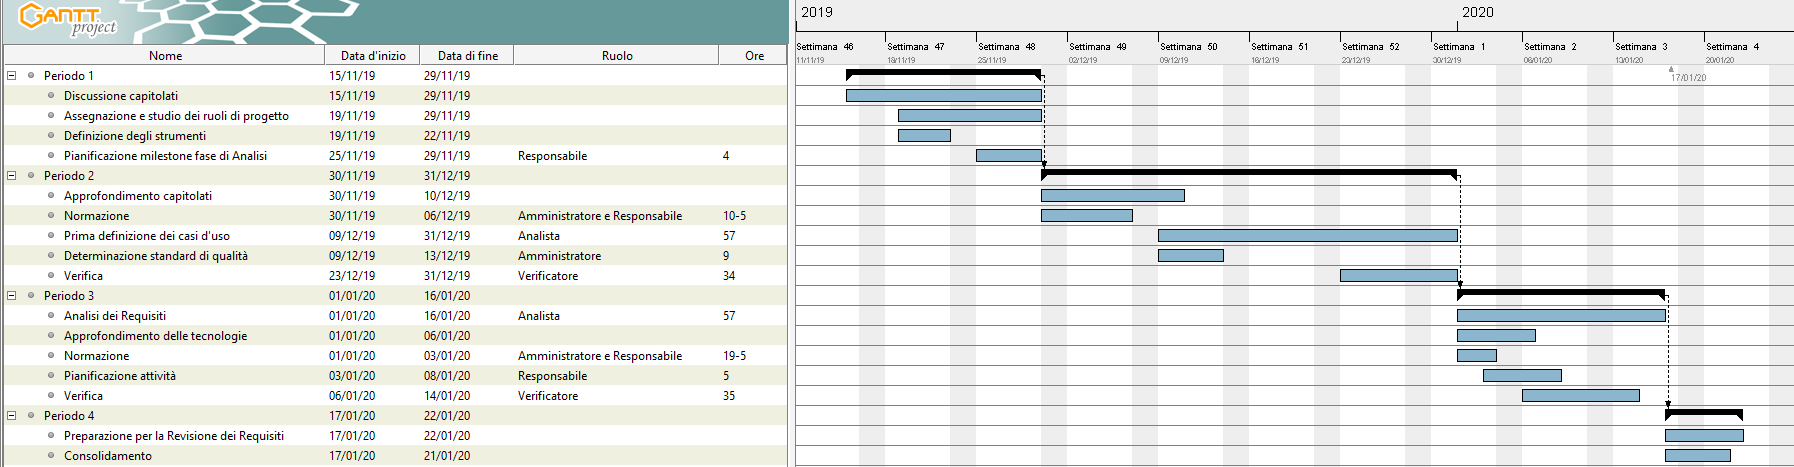
\includegraphics[scale=0.455]{Sezioni/DiagrammiGantt/Analisi.png}
	\caption{Diagramma di Gantt delle attività della fase di Analisi}
\end{figure}
\end{landscape}
\clearpage

\subsection{Progettazione Architetturale}
Periodo: dal 2020-01-22 al 2020-03-15\\
Inizia al termine della fase di Analisi e finisce con la data di consegna della Revisione di Progettazione.\\
In questa fase viene definita una soluzione architetturale in modo da soddisfare i requisiti individuati nella fase di Analisi.

\subsubsection{Periodo 1} 
Dal 2020-01-22 al 2020-02-11
\begin{itemize}
	\item \textbf{Normazione}: Standardizzazione e correzione di alcune parti dei documenti che non aderiscono completamente alle \NdP{};
	\item \textbf{Analisi dei requisiti}: Correzione e modifica dei casi d'uso segnalati;
	\item \textbf{Assegnazione dei ruoli di progetto}: Assegnazione dei ruoli di ciascun membro del gruppo in base alla suddivisione oraria indicata in §5.2.1;
	\item \textbf{Pianificazione attività}: Le attività da svolgere devono essere prima pianificate e discusse dal gruppo per garantire il \glo{way of working} sancito nelle \NdP{};
	\item \textbf{Approfondimento delle tecnologie}: Ricerca di documentazione e materiali utili per l'apprendimento delle nuove tecnologie da utilizzare per la realizzazione del prodotto finale;
	\item \textbf{Verifica}: Verifica dell'andamento del team in relazione alle tempistiche e allo svolgimento dei compiti assegnati.
\end{itemize}

\subsubsection{Periodo 2} 
Dal 2020-02-12 al 2020-03-08
\begin{itemize}
	\item \textbf{Studio delle tecnologie}: l'\glo{IaaS} \glo{Kubernetes} o i \glo{PaaS} \glo{Openshift} o \glo{Rancher}, \glo{LDAP} e \glo{GPS};
	\item \textbf{Normazione}: Decisioni ed inserimento delle nuove regole da adottare per le prossime condizioni dello sviluppo;
	\item \textbf{Miglioramento standard di qualità}: Aggiunta, rimozione o modifica di alcune metriche per garantire le qualità di processo e di prodotto affermate nel \PdQ{};
	\item \textbf{Technology Baseline}: Redazione della \glo{Technology Baseline}, cioè un allegato tecnico nel quale vengono indicate le tecnologie e i design pattern che vengono utilizzati durante lo sviluppo del prodotto;
	\item \textbf{Proof of Concept}: Creazione di un eseguibile che permetta di dimostrare la validità del prodotto che si vuole fornire, concretizzando la \glo{Technology Baseline};
	\item \textbf{Codifica}: Viene codificato il \glo{Proof of Concept} e successivamente condiviso tramite i \glo{repository} del gruppo al committente e al proponente in una data da definire;
	\item \textbf{Verifica}: Verifica dell'andamento del team in relazione alle tempistiche e allo svolgimento dei compiti assegnati.
\end{itemize}

\subsubsection{Periodo 3} 
Dal 2020-03-09 al 2020-03-15
\begin{itemize}
	\item \textbf{Consolidamento}: Ogni membro si prende del tempo per ripassare tutto il lavoro svolto e per studiare il necessario per affrontare al meglio le fasi successive;
	\item \textbf{Preparazione per la Revisione di Progettazione}: Il gruppo produce il materiale necessario da esporre alla presentazione pubblica della nostra proposta.
\end{itemize}

\newpage
% Inizia la pagina orientata orizzontalmente
\begin{landscape}
% Ora la pagina e' in orizzontale!
\subsubsection{Diagramma di Gantt delle attività della fase di Progettazione Architetturale}
\pagestyle{empty}
\begin{figure}[h]
	\centering
	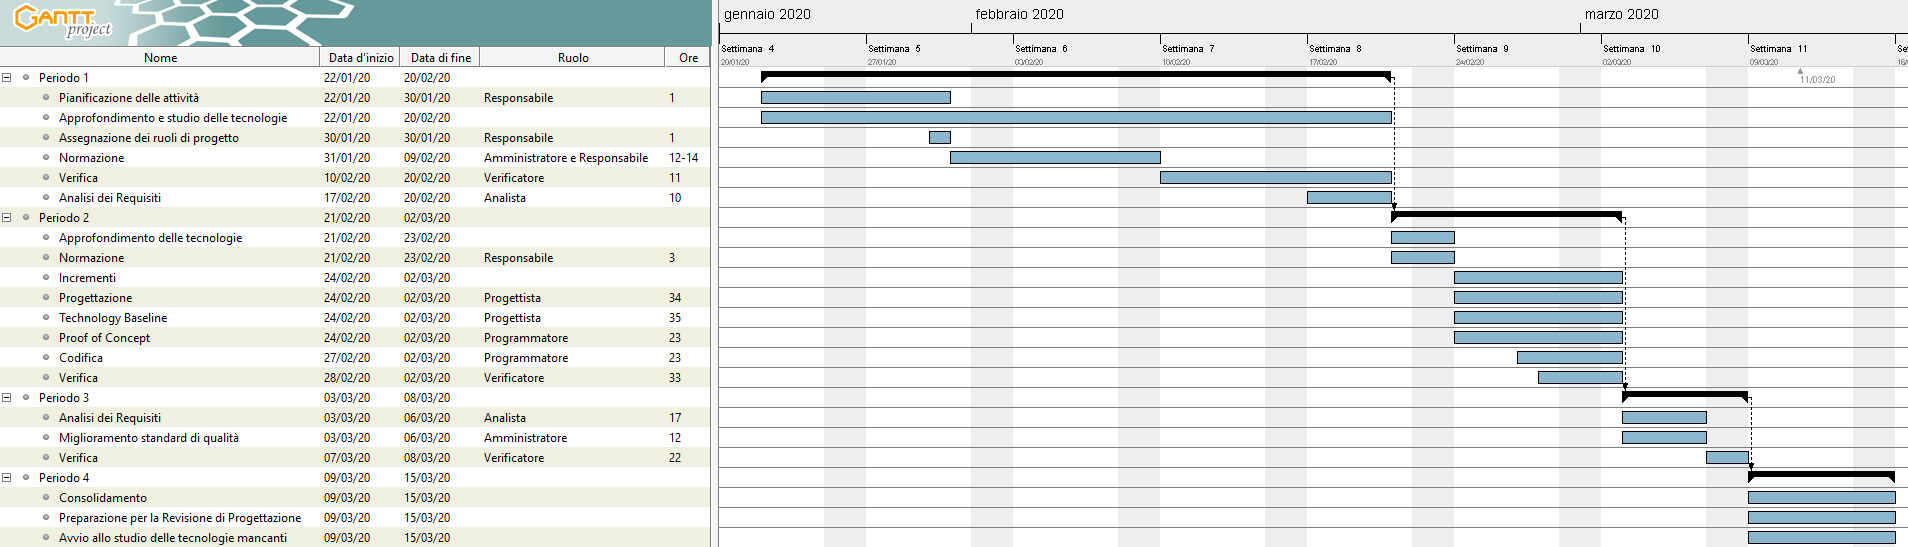
\includegraphics[scale=1.48]{Sezioni/DiagrammiGantt/ProgettazioneArchitetturale.png}
	\caption{Diagramma di Gantt delle attività della fase di Progettazione Architetturale}	
\end{figure}
\end{landscape}

\subsection{Progettazione di Dettaglio e Codifica}
Dal 2020-03-16 al 2020-04-19\\
Inizia al termine della fase di Progettazione Architetturale e finisce con la data di consegna della Revisione di Qualifica.\\
In questa fase si definisce nel dettaglio e si implementa l'architettura logica costruita nella fase di Progettazione Architetturale.

\subsubsection{Periodo 1} 
Dal 2020-03-16 al 2020-03-27\\
\begin{itemize}
	\item \textbf{Approfondimento delle tecnologie}: Ricerca di documentazione e materiali utili per l'apprendimento delle nuove tecnologie da utilizzare per la realizzazione del prodotto finale;
	\item \textbf{Normazione}: Standardizzazione e correzione di alcune parti dei documenti che non aderiscono completamente alle \NdP{};
	\item \textbf{Assegnazione dei ruoli di progetto}: Assegnazione dei ruoli di ciascun membro del gruppo in base alla suddivisione oraria indicata in §5.3.1;
	\item \textbf{Pianificazione delle attività}: Le attività da svolgere devono essere prima pianificate e discusse dal gruppo per garantire successivamente un buon \glo{way of working};
	\item \textbf{Progettazione}: Ricerca di una soluzione soddisfacente per tutti gli \glo{stakeholder}, descrive l'architettura del prodotto prima di pensare al codice ed attua un approccio sintetico;
	\item \textbf{Codifica}: Implementazione dei requisiti di base identificati per ottenere un sistema stabile;
	\item \textbf{Manuali}: Stesura del manuale utente e del manuale per il manutentore, in relazione alle funzionalità del sistema.
\end{itemize}
\subsubsection{Periodo 2} 
Dal 2020-03-28 al 2020-04-08\\
\begin{itemize}
	\item \textbf{Implementazione della Product Baseline:} Seguendo le specifiche della \glo{Technology Baseline};
	\item \textbf{Codifica incrementale:} Aggiunta di requisiti al sistema tramite incrementi;
	\item \textbf{Incremento e verifica:} Incrementi e verifiche con eventuali aggiunte al lavoro svolto in precedenza;
	\item \textbf{Manuali:} Aggiunta nel manuale utente e nel manuale manutentore delle funzionalità inserite incrementalmente nel sistema;
\end{itemize}
\subsubsection{Periodo 3}
Dal 2020-04-09 al 2020-04-12\\
\begin{itemize}
	\item \textbf{Primo rilascio del prodotto}: Pubblicazione del prodotto in un apposito \glo{repository} condiviso dai membri del gruppo;
	\item \textbf{Verifica}: Verifica dell'andamento del team in relazione alle tempistiche e allo svolgimento dei compiti assegnati;
\end{itemize}
\subsubsection{Periodo 4} 
Dal 2020-04-13 al 2020-04-19\\
\begin{itemize}
	\item \textbf{Consolidamento}: Ogni membro si prende del tempo per ripassare tutto il lavoro svolto e per studiare il necessario per affrontare al meglio le fasi successive;
	\item \textbf{Preparazione per la Revisione di Qualifica}: Il gruppo produce il materiale necessario da esporre alla presentazione pubblica della nostra proposta.
\end{itemize}

\newpage
% Inizia la pagina orientata orizzontalmente
\begin{landscape}
% Ora la pagina e' in orizzontale!
\subsubsection{Diagramma di Gantt delle attività della fase di Progettazione di Dettaglio e Codifica}
\pagestyle{empty}
\begin{figure}[h]
	\centering
	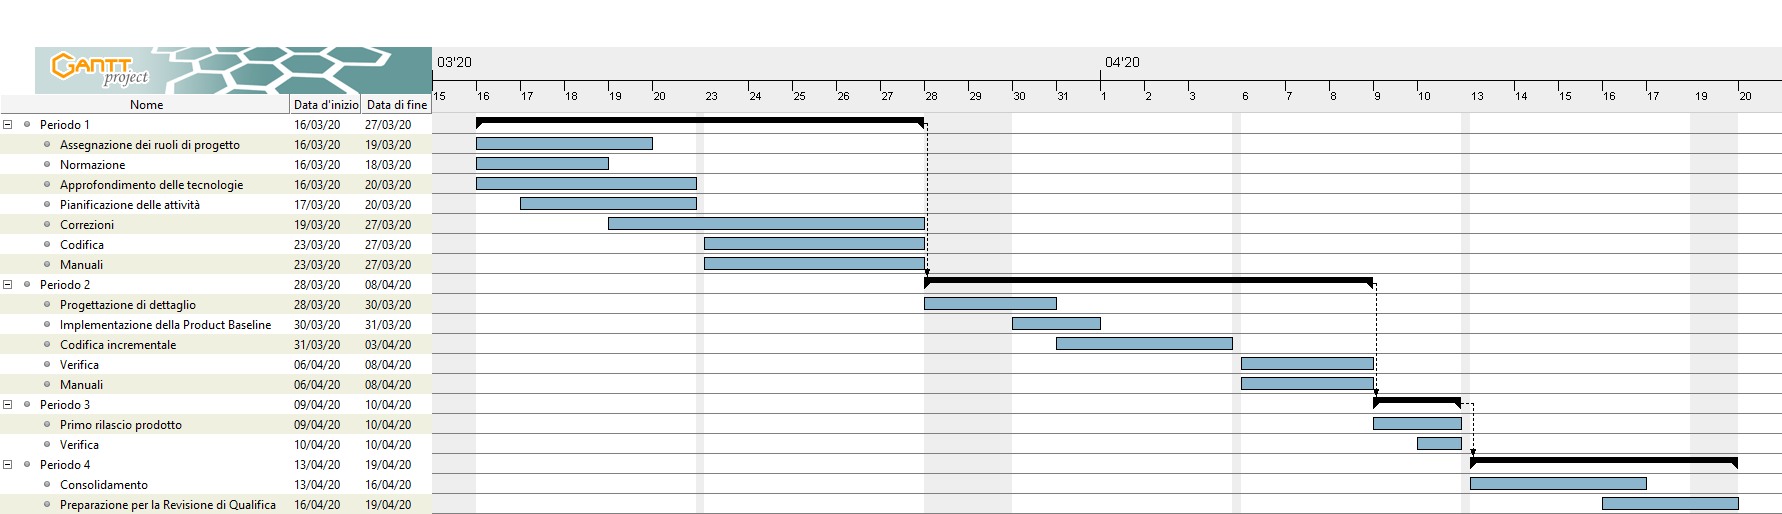
\includegraphics[scale=0.476]{Sezioni/DiagrammiGantt/ProgettazioneDiDettaglio.png}
	\caption{Diagramma di Gantt delle attività della fase di Progettazione di Dettaglio e Codifica}
\end{figure}
\end{landscape}

\subsection{Validazione e Collaudo}
Inizia al termine della progettazione di dettaglio e codifica e finisce con la data di consegna della revisione di accettazione.
\\In questo fase vengono definite le attività che servono per verificare che il prodotto corrisponde a quello desiderato dal cliente.
\subsubsection{Periodo 1} 
Dal 2020-04-21 al 2020-04-28
\begin{itemize}
	\item \textbf{Normazione:} Standardizzazione e correzione di alcune parti dei documenti che non aderiscono completamente alle norme;
	\item \textbf{Assegnazione dei ruoli di progetto:} Ad ogni membro del gruppo viene assegnato il ruolo principale da ricoprire nella fase di progettazione di validazione e collaudo;
	\item \textbf{Soddisfazione dei requisiti:} Controllo che i requisiti siano soddisfatti;
	\item \textbf{Pianificazione attività:} Le attività da svolgere devono essere prima pianificate e discusse dal gruppo per garantire successivamente un buon \glo{way of working};
	\item \textbf{Verifica} Verifica dell'andamento del team in relazione alle tempistiche e allo svolgimento dei compiti assegnati.
\end{itemize}
\subsubsection{Periodo 2} 
Dal 2020-04-29 al 2020-05-10
\begin{itemize}
	\item \textbf{Codifica:} Esecuzione dell'ultimo versionamento del prodotto;
	\item \textbf{Verifica:} Accertamento che le esecuzioni delle attività siano esenti da errori;
	\item \textbf{Validazione:} Verifica se il prodotto realizzato sia conforme alle attese, e validazione finale in caso di esito positivo;
	\item \textbf{Scrittura dei manuali:} Esecuzione del secondo versionamento del manuale utente e del manuale manutentore;
	\item \textbf{Collaudo:} Vengono eseguiti gli ultimi test sul prodotto per verificare se le funzionalità rispettano i risultati attesi.
\end{itemize}
\subsubsection{Periodo 3} 
Dal 2020-05-11 al 2020-05-17
\begin{itemize}
	\item \textbf{Preparazione per la Revisione di Accettazione:} Il gruppo produce il materiale necessario da esporre alla presentazione pubblica della nostra proposta.
\end{itemize}


\newpage
% Inizia la pagina orientata orizzontalmente
\begin{landscape}
	% Ora la pagina e' in orizzontale!
	\subsubsection{Diagramma di Gantt delle attività}
	\pagestyle{empty}
	\begin{figure}[h]
		
		\begin{center}	
			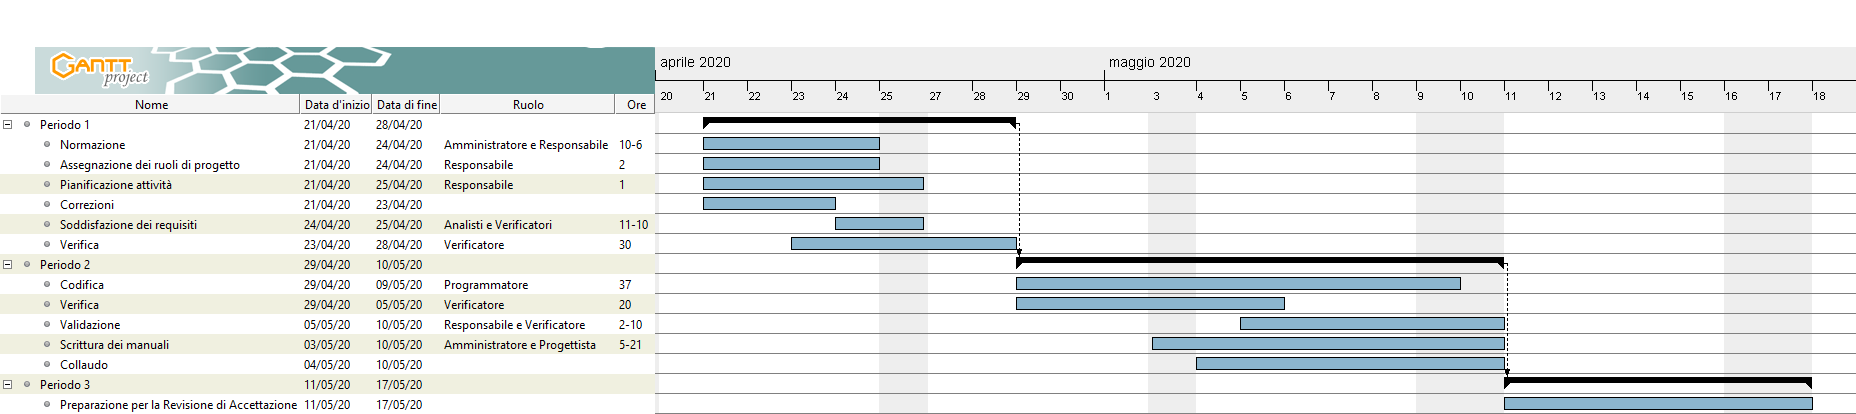
\includegraphics[scale=1.6]{Sezioni/DiagrammiGantt/Validazione.png}
		\end{center}
	\caption{Diagramma di Gantt delle attività di Validazione e Collaudo}	
	\end{figure}
\end{landscape}